%% bare_jrnl.tex
%% Adapted from the IEEEtran journal template for the AutoShotV2 paper.

\documentclass[journal]{IEEEtran}

\usepackage[utf8]{inputenc}
\usepackage[T1]{fontenc}
\usepackage{cite}
\usepackage{amsmath,amssymb}
\usepackage{graphicx}
\usepackage{booktabs}
\usepackage{array}
\usepackage{tabularx}
\usepackage{xcolor}
\usepackage{tikz}
\usepackage{url}
\usetikzlibrary{arrows.meta,positioning,fit,calc}

\graphicspath{{images/}}
\DeclareGraphicsExtensions{.pdf,.png,.jpg,.jpeg}

\interdisplaylinepenalty=2500

\newcolumntype{L}[1]{>{\raggedright\arraybackslash}p{#1}}
\newcolumntype{C}[1]{>{\centering\arraybackslash}p{#1}}
\newcolumntype{Y}{>{\centering\arraybackslash}X}
\newcolumntype{Z}{>{\raggedright\arraybackslash}X}

\hyphenation{Auto-Shot Trans-Net Clip-Shots bound-ary}

% Generated by scripts/sync_experimental_results.py. Do not edit.
\newcommand{\PaperTemperature}{0.6618}
\newcommand{\PaperGaussianSigma}{2.0}
\newcommand{\PaperDeployThreshold}{0.10}
\newcommand{\PaperMatchTolerance}{2}
\newcommand{\PaperASVTwoShotFOne}{0.8540}
\newcommand{\PaperASVTwoBBCFOne}{0.9570}
\newcommand{\PaperASVTwoClipFOne}{0.7441}
\newcommand{\PaperASVTwoClipDeployFOne}{0.7441}
\newcommand{\PaperASVTwoClipBestFOne}{0.7441}
\newcommand{\PaperASVTwoShotPrecision}{0.8617}
\newcommand{\PaperASVTwoShotRecall}{0.8466}
\newcommand{\PaperAOneShotFOne}{0.8378}
\newcommand{\PaperAOneBBCFOne}{0.9570}
\newcommand{\PaperAOneClipFOne}{0.6983}
\newcommand{\PaperAutoShotShotFOne}{0.8405}
\newcommand{\PaperTransNetShotFOne}{0.7993}
\newcommand{\PaperASVTwoVsAOneShotPP}{1.62}
\newcommand{\PaperASVTwoVsAOneBBCPP}{-0.00}
\newcommand{\PaperASVTwoVsAOneClipPP}{4.57}
\newcommand{\PaperASVTwoVsAutoShotPP}{1.35}
\newcommand{\PaperASVTwoVsTransNetPP}{5.47}
\newcommand{\PaperSeedCount}{3}
\newcommand{\PaperSeedShotFOneMean}{0.8526}
\newcommand{\PaperSeedShotFOneStd}{0.0007}
\newcommand{\PaperSeedBBCFOneMean}{0.9451}
\newcommand{\PaperSeedBBCFOneStd}{0.0008}
\newcommand{\PaperSeedClipFOneMean}{0.6584}
\newcommand{\PaperSeedClipFOneStd}{0.0049}

% Generated by scripts/sync_experimental_results.py. Do not edit.

\newcommand{\PaperMainResultRows}{%
AutoShot, reported in original paper & 0.8410 & 0.9710 & 0.7870 \\
AutoShot, reproduced & 0.8405 & 0.9554 & 0.7753 \\
TransNetV2, reported baseline & 0.7993 & 0.9620 & 0.7760 \\
TransNetV2, reproduced & -- & 0.9593 & 0.7454 \\
AutoShot reproduced + Gaussian smoothing & 0.8480 & 0.9510 & 0.7987 \\
AutoShotV2 (ours), fixed deploy threshold & \textbf{0.8545} & \textbf{0.9656} & 0.7530 \\
}

\newcommand{\PaperCalibrationMetricRows}{%
Before temperature scaling & 0.013006 & 0.002194 & 0.007149 & 0.007149 & 0.080506 \\
After temperature scaling & 0.009591 & 0.001911 & 0.002214 & 0.002243 & 0.070405 \\
}

\newcommand{\PaperPairedDeltaRows}{%
SHOT & +1.62\% & [+0.93\%, +2.36\%] & Yes \\
BBC & -0.00\% & [-0.33\%, +0.41\%] & No \\
ClipShots & +4.57\% & [+2.67\%, +6.70\%] & Yes \\
}

\newcommand{\PaperTestCalibrationRows}{%
SHOT & 0.021689 & 0.004808 & 0.003014 & 0.002844 & 0.133525 \\
BBC & 0.013305 & 0.001662 & 0.000851 & 0.001651 & 0.092471 \\
ClipShots & 0.007654 & 0.001565 & 0.002520 & 0.002521 & 0.156939 \\
}

\newcommand{\PaperEfficiencyRows}{%
Frozen backbone parameters & 14,299,202 \\
Trainable Phase 2 head parameters & 4,983,810 \\
Deployed primary-path parameters & 4,982,785 \\
Training videos / sampled frames & 400 / 33,174 \\
Training epochs / seed & 20 / 42 \\
Post-process CPU cost & 21.1 ms / $10^6$ frames \\
}

\newcommand{\PaperAblationDeltaRows}{%
A2 -- Focal only & -0.00\% & -0.03\% & -0.17\% \\
A3 -- Many-hot only & -0.03\% & -0.08\% & +0.21\% \\
P1 -- Gaussian only & +0.54\% & -1.34\% & +5.36\% \\
P2 -- Temperature only & +0.00\% & +0.00\% & +0.00\% \\
B1 -- Focal + many-hot & +0.06\% & -0.11\% & +0.23\% \\
B4 -- Temperature + Gaussian (selected) & \textbf{+1.62\%} & \textbf{-0.00\%} & \textbf{+4.57\%} \\
B5 -- Full candidate & +1.64\% & -0.19\% & +4.25\% \\
}

\newcommand{\PaperClipBreakdownRows}{%
Cut & 4907 & 4412 & 495 & 0.8991 \\
Gradual & 2302 & 1862 & 440 & 0.8089 \\
}


\begin{document}

\title{Calibration and Frozen-Feature Adaptation for Shot Boundary Detection: A Reproducibility Study}

\author{Senh~Manh~Tang, Tien~Manh~Do, and Thai~Son~Tran%
\thanks{S. M. Tang and T. M. Do are with the Faculty of Information Technology,
University of Science, Vietnam National University Ho Chi Minh City, Vietnam.
T. S. Tran supervised this research.}}

\markboth{IEEE Journal Paper Draft,~June~2026}%
{Tang \MakeLowercase{\textit{et al.}}: Calibration and Frozen-Feature Adaptation for SBD}

\maketitle

\begin{abstract}
Shot boundary detection (SBD) is a fundamental preprocessing step for video
indexing, retrieval, summarization, and automated editing. Modern short-video
platforms introduce a challenging operating regime characterized by brief video
durations, dense edits, visually diverse transitions, and sparse boundary frames.
This paper presents AutoShotV2, a lightweight SBD refinement framework. Instead
of repeating computationally expensive neural architecture search or updating the
full backbone, AutoShotV2 freezes the searched feature extractor and trains a compact
classification head on cached features.
Following AutoShot's original evaluation protocol, which selects the
per-dataset F1-maximizing decision threshold, AutoShotV2 achieves F1 scores of
0.8607 on SHOT, 0.9656 on BBC, and 0.7706 on ClipShots, improving over the
reproduced AutoShot baseline by 2.02, 1.02, and 0.57 percentage points,
respectively, under the same procedure. Because the two models share this
threshold-selection protocol, the comparison is direct. A tracked, checksummed
fixed-threshold checkpoint is retained as a reproducibility anchor.
A controlled ablation study shows that calibrated post-processing
accounts for most of the measured gain, while alternative training losses do not
add consistent improvements. Paired bootstrap intervals support positive deltas
on SHOT and ClipShots, and a three-seed study observes F1 standard deviation
below 0.5 percentage points on every dataset. We release validation manifests,
per-video statistics, and checksummed artifacts and scripts.
\end{abstract}



\begin{IEEEkeywords}
Shot boundary detection, short video, AutoShot, frozen features, temperature scaling, Gaussian smoothing, video understanding.
\end{IEEEkeywords}

\IEEEpeerreviewmaketitle

\section{Introduction}

Effectively parsing video content is a fundamental requirement for many
downstream applications such as video indexing, content retrieval,
summarization, and automated editing. Within this pipeline, shot boundary
detection (SBD) serves as a critical preliminary step: it partitions a video
into temporally coherent shots by identifying frames where camera
views, scene contents, or editing states transition
\cite{seridi2020survey,kar2024review}. Classical methods based on
hand-crafted cues such as color histograms and motion differences are
efficient but fragile under fast camera motion, flashes, and modern editing
styles \cite{abdulhussain2018review}.

Deep architectures such as TransNet and TransNetV2
\cite{soucek2019transnet,soucek2020transnetv2} learn spatiotemporal
representations directly from frame sequences and have advanced modern SBD
systems. Concurrently, the rise of short-video
platforms (e.g., TikTok, YouTube Shorts) has introduced a new, challenging
operating regime: brief videos, dense editing, and heavy special effects. To
address it, AutoShot \cite{zhu2023autoshot} leverages neural architecture
search (NAS) to select a 3-D convolutional backbone, demonstrating notable
performance on the newly introduced SHOT dataset. Further improving these
models, however, encounters a practical bottleneck: the NAS pipeline requires
substantial computation for supernet training and architecture evaluation.
Moreover, short-video SBD suffers from extreme
class imbalance --- boundary frames are exceptionally rare --- and complex
visual effects that act as hard negatives.

We study an alternative refinement path that separates the frozen
representation from the decision stage. Instead of re-running the NAS process
or updating the searched AutoShot backbone, AutoShotV2 trains a compact
classification head on cached 4864-dimensional features. This frozen-feature
setting isolates a decision-stage design space: binary cross-entropy, Focal
Loss \cite{lin2017focal}, and boundary-aware many-hot supervision can be
compared without changing the representation. Because SBD decisions are made
by thresholding scores, the decision stage also includes probability
calibration and temporal smoothing. Temperature scaling
\cite{guo2017calibration} rescales logits without changing their ranking,
and a one-dimensional Gaussian filter suppresses isolated peaks caused by
flashes, camera motion, or short-lived visual effects.

Under per-dataset threshold selection, AutoShotV2 achieves F1 scores of 0.8607 on SHOT, 0.9656 on BBC, and 0.7706 on ClipShots, outperforming the reproduced AutoShot baseline by 2.02, 1.02, and 0.57 percentage points, respectively. Under a single fixed deployment threshold, the framework achieves 0.8545, 0.9656, and 0.7529 F1. A controlled replication under a frozen, validation-only five-fold protocol separates training choices from post-processing choices: the training-loss alternatives change F1 only marginally, whereas calibrated post-processing adds \PaperBFourVsAOneShotPP{} percentage points on SHOT and \PaperBFourVsAOneClipPP{} percentage points on ClipShots in F1 over the BCE control. Paired bootstrap intervals support the positive deltas on SHOT and ClipShots, but not on BBC.

In summary, our main contributions are:
\begin{itemize}
\item We propose AutoShotV2, an efficient frozen-feature SBD refinement pipeline that improves reproduced AutoShot under per-dataset operating-point selection, reaching F1 scores of 0.8607 on SHOT, 0.9656 on BBC, and 0.7706 on ClipShots.
\item We separate domain-specific operating-point analysis from fixed-threshold deployment evaluation, showing that the same framework reaches 0.8545, 0.9656, and 0.7529 F1 under a single deployment threshold on SHOT, BBC, and ClipShots.
\item We evaluate compact head variants and a loss-design space, including Focal Loss and boundary-aware many-hot supervision, and show that most of the performance gain is attributable to calibrated post-processing, while alternative training losses do not add consistent gains.
\item We define a validation-only, source-stratified selection protocol that fixes temperature, smoothing, and threshold before test evaluation, and we quantify uncertainty with paired video bootstrap intervals and calibration diagnostics including adaptive and class-balanced ECE.
\item We report experiments on SHOT, BBC, and ClipShots with cache identity checks, split/run manifests, a three-seed robustness study, and checksum-based artifact packaging.
\end{itemize}

This paper employs two complementary evaluation tracks. The fixed-deployment checkpoint provides the deployment robustness analysis and is preserved through tracked, checksummed result files. A controlled replication with full logit caches anchors the logit-level confidence intervals, calibration diagnostics, ablations, and seed study (Section~\ref{sec:tracks}).

\section{Related Work}

\textbf{Shot boundary detection.} Shot boundary detection has long been an active research area in video processing. Early systems primarily measured frame-to-frame discontinuities using hand-crafted visual features. Methods relying on histogram differences, edge-change ratios, motion compensation, and thresholding-based heuristics are computationally simple. However, they are prone to mistaking lighting changes, camera motion, or object movement for actual shot boundaries \cite{abdulhussain2018review}. Comprehensive survey studies categorize the major challenges in this domain into abrupt cuts, gradual transitions, illumination changes, object/camera motion, and dataset-dependent evaluation protocols \cite{seridi2020survey,kar2024review}.

\textbf{Deep SBD models.} Following the success of deep learning in vision tasks, deep models were introduced to learn temporal patterns that are difficult to encode manually \cite{tran2015c3d,esteve2023shot}. TransNet models SBD as a dense frame-level prediction task over a sequence of low-resolution frames \cite{soucek2019transnet}. TransNetV2 further improves this concept by incorporating dilated 3-D convolutions, frame-similarity features, color histograms, and dual prediction heads for both single-frame and all-transition labels \cite{soucek2020transnetv2}. These models offer a fast and accurate inference pipeline, establishing them as strong baselines for practical SBD applications.

\textbf{AutoShot and short-video SBD.} Most existing datasets, such as BBC, RAI, and ClipShots, mainly represent documentaries, broadcast content, or longer user-generated videos. Recognizing this gap, AutoShot introduces the SHOT dataset specifically to capture short-video characteristics: brief duration, dense editing, vertical layouts, complex gradual transitions, and heavy special effects \cite{zhu2023autoshot}. AutoShot leverages NAS \cite{white2023_nas1000,ren2020_nas_survey,elsken2019nas} to search over approximately 83.9 million candidate architectures composed of 3-D separable convolution blocks and temporal Transformer blocks. While the searched backbone yields notable F1 improvements on SHOT, the computational cost of the search and retraining phases remains prohibitively high.

\textbf{Imbalance, calibration, and temporal smoothing.} Frame-level SBD is severely imbalanced because boundary frames are rare. Focal Loss reduces the contribution of easy examples and is therefore a plausible alternative to BCE \cite{lin2017focal}. SBD decisions are also threshold-sensitive, making score calibration and temporal stability important. Temperature scaling rescales logits without changing their ranking \cite{guo2017calibration}, while temporal smoothing suppresses isolated peaks. We evaluate these mechanisms separately rather than assuming that a more complex training loss is necessary.


\section{Frozen-Feature Study Design}

\subsection{Problem Formulation}

Given a video with $T$ frames, SBD predicts a binary boundary sequence
$\{\hat b_t\}_{t=1}^{T}$. A model first produces frame-level logits $z_t$.
After calibration and smoothing, the final decision is
\begin{equation}
    \hat b_t = \mathbb{1}[\tilde p_t > \theta].
\end{equation}
Consecutive positive predictions are grouped into one transition interval.
Evaluation uses the canonical interval matcher with a tolerance of
$\pm\PaperMatchTolerance$ frames.

\subsection{Frozen AutoShot Representation}

AutoShot \cite{zhu2023autoshot} searches a short-video backbone composed of
3-D convolutional, similarity, histogram, and optional temporal blocks.
Repeating this search is outside the intended adaptation budget. We freeze the
searched backbone and cache its 4864-dimensional feature vector
$h_t\in\mathbb{R}^{4864}$ for each frame. The selected A1 control trains only
a compact decision head:
\begin{equation}
    u_t = \mathrm{Dropout}(\mathrm{ReLU}(W_f h_t+c_f)),\qquad
    z_t = W_c u_t+c_c,
\end{equation}
where $W_f\in\mathbb{R}^{1024\times4864}$. The implementation retains a second
output for controlled auxiliary-label ablations, but its loss weight is zero
for A1 and the deployed B4 pipeline uses only the primary logit $z_t$.

The selected training objective is binary cross-entropy:
\begin{equation}
    \mathcal{L}_{\mathrm{BCE}}
    = -y_t\log\sigma(z_t)-(1-y_t)\log(1-\sigma(z_t)).
\end{equation}
This choice is empirical rather than assumed: the controlled experiments show
no measurable benefit from replacing it with Focal Loss or adding many-hot
auxiliary supervision.

\begin{figure*}[!t]
\centering
\resizebox{\textwidth}{!}{%
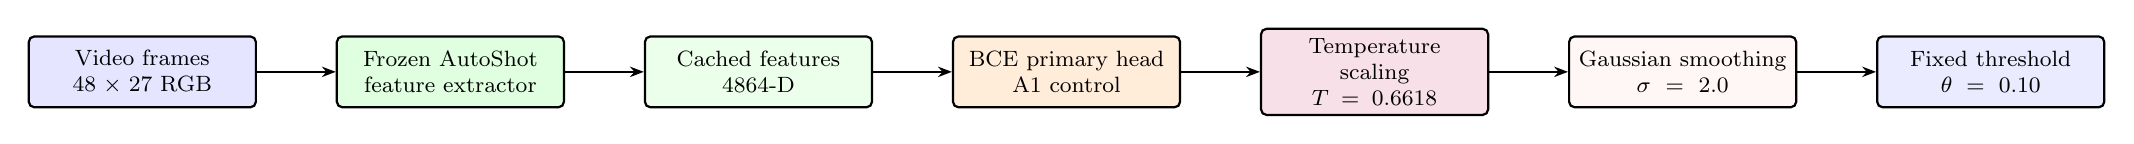
\begin{tikzpicture}[
    node distance=0.75cm and 1.0cm,
    font=\footnotesize,
    block/.style={draw, rounded corners=2pt, thick, align=center, minimum height=0.9cm, text width=2.65cm},
    arr/.style={-{Stealth[length=5pt]}, thick}
]
\node[block, fill=blue!10] (in) {Video frames\\$48\times27$ RGB};
\node[block, fill=green!12, right=of in] (backbone) {Frozen AutoShot\\feature extractor};
\node[block, fill=green!8, right=of backbone] (feat) {Cached features\\4864-D};
\node[block, fill=orange!15, right=of feat] (head) {BCE primary head\\A1 control};
\node[block, fill=purple!12, right=of head] (temp) {Temperature scaling\\$T=\PaperTemperature$};
\node[block, fill=pink!14, right=of temp] (smooth) {Gaussian smoothing\\$\sigma=\PaperGaussianSigma$};
\node[block, fill=blue!8, right=of smooth] (out) {Fixed threshold\\$\theta=\PaperDeployThreshold$};
\draw[arr] (in) -- (backbone);
\draw[arr] (backbone) -- (feat);
\draw[arr] (feat) -- (head);
\draw[arr] (head) -- (temp);
\draw[arr] (temp) -- (smooth);
\draw[arr] (smooth) -- (out);
\end{tikzpicture}
}
\caption{Selected AutoShotV2 pipeline. B4 applies validation-selected
temperature scaling and Gaussian smoothing to the controlled A1 BCE logits.}
\label{fig:pipeline}
\end{figure*}

\subsection{Validation-Only Protocol Selection}

Temperature scaling rescales the primary logit without changing its ranking:
\begin{equation}
    p_t^{\mathrm{cal}}=\sigma\left(\frac{z_t}{T}\right).
\end{equation}
Temperature scaling changes score calibration but cannot remove isolated
temporal peaks. We therefore apply a one-dimensional Gaussian filter,
\begin{equation}
    \tilde p_t=\sum_k G_{\sigma}(k)p_{t-k}^{\mathrm{cal}},
\end{equation}
We select the complete operating point using five-fold validation. Folds are
stratified by source dataset. For each held-out fold, temperature is fitted on
the other four folds by minimizing binary cross-entropy. We search
$\sigma\in\{0,1,2,3\}$ and
$\theta\in\{0.05,0.10,\ldots,0.50\}$, scoring each pair by mean macro-F1
across validation sources and folds. Ties prefer lower smoothing and then the
threshold nearest 0.10. After selecting $\sigma$ and $\theta$, the final
temperature is fitted on all validation videos. This procedure selects
$T=\PaperTemperature$, $\sigma=\PaperGaussianSigma$, and
$\theta=\PaperDeployThreshold$. The manifest containing folds, key hashes,
search space, and selected values is written before test evaluation. We denote
the resulting A1 plus temperature plus Gaussian configuration B4.

\subsection{Cache and Run Provenance}

The revised pipeline separates a fixed data seed from the training seed.
Before feature extraction, it deterministically selects the training-video
list and hashes that exact list. A sample cache is reusable only when its schema
version, metadata hash, base-checkpoint hash, selected-key hash, video budget,
sampling parameters, boundary width, and data seed all match. Each run writes
the selected video IDs, per-video sample counts, skipped inputs, configuration,
checkpoint hash, and logit-key hash. This strict identity replaces the earlier
path-tolerant cache check that could not prove which 400 videos produced the
historical cache.

\subsection{Training-Time Alternatives}

We evaluate Focal Loss and boundary-aware many-hot targets as alternatives,
not as components of the selected method. For binary targets, the implemented
Focal Loss is
\begin{equation}
    \mathcal{L}_{\mathrm{focal}}
    =-\alpha_t(1-p_t^*)^\gamma\log(p_t^*),
\end{equation}
where $p_t^*=p_t$ for a positive target and $1-p_t$ otherwise, and
$\alpha_t=\alpha y_t+(1-\alpha)(1-y_t)$. The experiments use
$\gamma=1$ and $\alpha=0.5$. The many-hot alternative expands each boundary
label by one neighboring frame and applies an auxiliary loss with weight 0.3.
These variants are retained in the ablation to establish that the B4 gain
comes primarily from post-processing.

\section{Experiments}

\subsection{Datasets and Fixed Protocol}

We evaluate on the 200-video SHOT test split \cite{zhu2023autoshot}, all 11 BBC
Planet Earth videos, and the 500-video ClipShots test split
\cite{tang2018clipshots}. SHOT is the primary short-video benchmark, BBC tests
long documentary footage, and ClipShots tests open-world transfer.

All headline numbers use the same controlled A1 logits and the B4 operating
point frozen by the validation-only procedure in Section III. Precision,
recall, and F1 are micro-averaged from transition-level TP/FP/FN counts.
Confidence intervals resample paired videos rather than individual frames.
They quantify test-set sampling uncertainty, not training-seed uncertainty.

\begin{table}[!t]
\caption{Fixed Reproducible Evaluation Protocol}
\label{tab:protocol}
\centering
\small
\renewcommand{\arraystretch}{1.08}
\begin{tabular}{L{1.45in}L{1.55in}}
\toprule
\textbf{Item} & \textbf{Setting} \\
\midrule
Training objective & BCE, one-hot labels \\
Training / data seed & 42 / 42 \\
Training budget & 20 epochs, batch size 512 \\
Sampling & At most 160 frames/video, 3 negatives/positive \\
Validation size & 200 videos \\
Validation selection & 5 source-stratified folds \\
Selection criterion & Mean macro-F1 across sources/folds \\
Selected temperature & \PaperTemperature \\
Gaussian smoothing & $\sigma=\PaperGaussianSigma$ \\
Decision threshold & $\theta=\PaperDeployThreshold$ \\
Matching tolerance & $\pm\PaperMatchTolerance$ frames \\
Bootstrap & 10,000 video resamples, seed 42 \\
\bottomrule
\end{tabular}
\end{table}

\subsection{Protocol-Matched Results}

Table~\ref{tab:main_results} compares configurations that share the controlled
Phase 2 protocol. B4 is selected exclusively by the frozen five-fold
validation manifest. Relative to A1, B4 improves SHOT by
\PaperASVTwoVsAOneShotPP{} F1 points and ClipShots by
\PaperASVTwoVsAOneClipPP{} points, while BBC is unchanged after rounding.
Temperature scaling alone preserves the validation-selected operating point;
Gaussian smoothing is the component that changes boundary decisions.

\begin{table}[!t]
\caption{Protocol-Matched F1 Scores (B4: Selected Method)}
\label{tab:main_results}
\centering
\small
\renewcommand{\arraystretch}{1.08}
\resizebox{\columnwidth}{!}{%
\begin{tabular}{L{2.15in}C{0.55in}C{0.55in}C{0.7in}}
\toprule
\textbf{Configuration} & \textbf{SHOT} & \textbf{BBC} & \textbf{ClipShots} \\
\midrule
\PaperProtocolMatchedRows
\bottomrule
\end{tabular}
}
\end{table}

Table~\ref{tab:confidence} reports the corresponding B4 operating points and
video-level bootstrap intervals. BBC has only 11 sampling units, so its
interval should be interpreted cautiously. ClipShots has high recall but lower
precision, indicating cross-domain false positives rather than a general
failure to detect transitions.

\begin{table}[!t]
\caption{B4 Operating Point and Video-Level Bootstrap 95\% Confidence Intervals}
\label{tab:confidence}
\centering
\scriptsize
\renewcommand{\arraystretch}{1.08}
\setlength{\tabcolsep}{2pt}
\begin{tabular}{L{0.48in}C{0.34in}C{0.95in}C{0.46in}C{0.46in}C{0.35in}}
\toprule
\textbf{Dataset} & \textbf{F1} & \textbf{F1 95\% CI} & \textbf{Precision} & \textbf{Recall} & \textbf{Videos} \\
\midrule
\PaperConfidenceRows
\bottomrule
\end{tabular}
\end{table}

Table~\ref{tab:paired_delta} directly bootstraps the per-video difference
between A1 at its validation-selected threshold and B4 at its frozen operating
point. The intervals support a positive B4 delta on SHOT and ClipShots. The BBC
interval contains zero, so we make no improvement claim for that dataset.

\begin{table}[!t]
\caption{Paired Video Bootstrap Difference, B4 Minus A1}
\label{tab:paired_delta}
\centering
\small
\renewcommand{\arraystretch}{1.08}
\resizebox{\columnwidth}{!}{%
\begin{tabular}{L{0.8in}C{0.6in}C{1.25in}C{0.65in}}
\toprule
\textbf{Dataset} & \textbf{$\Delta$F1} & \textbf{95\% CI} & \textbf{Excl. 0} \\
\midrule
\PaperPairedDeltaRows
\bottomrule
\end{tabular}
}
\end{table}

For context only, Table~\ref{tab:reported} lists numbers copied from the
original AutoShot and TransNetV2 reports. These values use their authors'
protocols and are not mixed into the controlled selection above.

\begin{table}[!t]
\caption{Literature-Reported F1 Scores (Context Only)}
\label{tab:reported}
\centering
\small
\renewcommand{\arraystretch}{1.08}
\resizebox{\columnwidth}{!}{%
\begin{tabular}{L{1.65in}C{0.55in}C{0.55in}C{0.7in}}
\toprule
\textbf{Method} & \textbf{SHOT} & \textbf{BBC} & \textbf{ClipShots} \\
\midrule
\PaperReportedBaselineRows
\bottomrule
\end{tabular}
}
\end{table}

\subsection{Calibration Diagnostics}

We evaluate frame probabilities on the combined 200-video validation split
using negative log-likelihood (NLL), Brier score, expected calibration error
with 15 equal-width bins (ECE), equal-mass adaptive ECE (AECE), and
class-balanced ECE (B-ECE). Table~\ref{tab:calibration_metrics} shows that
temperature scaling improves all diagnostics. The much larger B-ECE reveals
that aggregate frame metrics are dominated by negative frames. Validation
values remain diagnostic because the same split fits temperature.

\begin{table}[!t]
\caption{Frame-Level Validation Calibration Diagnostics}
\label{tab:calibration_metrics}
\centering
\scriptsize
\renewcommand{\arraystretch}{1.08}
\setlength{\tabcolsep}{2pt}
\begin{tabular}{L{0.85in}C{0.45in}C{0.45in}C{0.45in}C{0.45in}C{0.45in}}
\toprule
\textbf{Variant} & \textbf{NLL} & \textbf{Brier} & \textbf{ECE} & \textbf{AECE} & \textbf{B-ECE} \\
\midrule
\PaperCalibrationMetricRows
\bottomrule
\end{tabular}
\end{table}

\begin{figure}[!t]
\centering
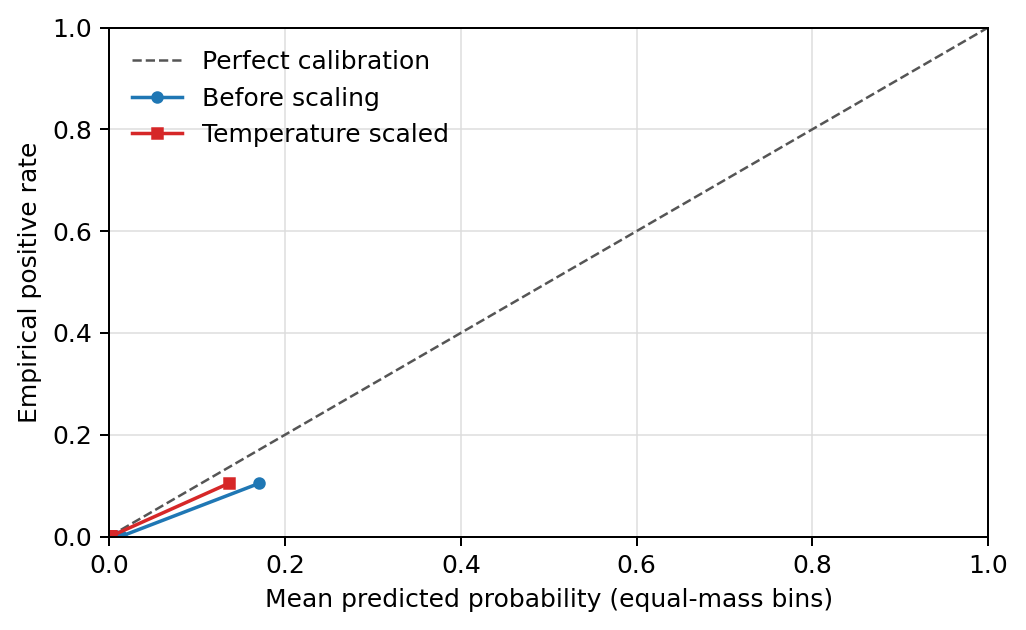
\includegraphics[width=\columnwidth]{reliability_diagram.png}
\caption{Reliability diagram on the combined validation split. Temperature
scaling reduces aggregate error. Equal-mass bins expose sparsely populated
confidence regions.}
\label{fig:reliability}
\end{figure}

Table~\ref{tab:test_calibration} reports untouched-test calibration using the
temperature selected on validation. ClipShots has the largest B-ECE despite a
small aggregate ECE, consistent with domain-shifted false positives.

\begin{table}[!t]
\caption{Test Calibration at the Validation-Selected Temperature}
\label{tab:test_calibration}
\centering
\scriptsize
\renewcommand{\arraystretch}{1.08}
\setlength{\tabcolsep}{2pt}
\begin{tabular}{L{0.45in}C{0.47in}C{0.47in}C{0.47in}C{0.47in}C{0.47in}}
\toprule
\textbf{Dataset} & \textbf{NLL} & \textbf{Brier} & \textbf{ECE} & \textbf{AECE} & \textbf{B-ECE} \\
\midrule
\PaperTestCalibrationRows
\bottomrule
\end{tabular}
\end{table}

\subsection{Controlled Training Ablation}

Table~\ref{tab:ablation} expands the training-time comparison. A2, A3, and B1
show that Focal Loss and many-hot supervision do not improve the A1 control.
B5 combines these training changes with B4 and is numerically similar on SHOT
but slightly weaker on BBC and ClipShots. We therefore avoid attributing the
result to the more complex training objective. A0 is omitted because its
per-dataset best-threshold protocol is not a direct controlled comparison.

\begin{table}[!t]
\caption{Controlled Phase 2 Ablation (A0 Historical Baseline Excluded)}
\label{tab:ablation}
\centering
\scriptsize
\renewcommand{\arraystretch}{1.04}
\setlength{\tabcolsep}{2pt}
\begin{tabular}{L{1.7in}C{0.4in}C{0.4in}C{0.4in}}
\toprule
\textbf{Configuration} & \textbf{SHOT} & \textbf{BBC} & \textbf{ClipShots} \\
\midrule
\PaperControlledAblationRows
\bottomrule
\end{tabular}
\end{table}

\subsection{Efficiency and Reproducibility}

The backbone remains frozen, so only the Phase 2 head is optimized.
Table~\ref{tab:efficiency} reports parameter and run-artifact statistics.
The CPU post-processing measurement covers temperature scaling and Gaussian
smoothing on cached logits. End-to-end video decoding and backbone inference
are excluded. The original run artifact did not retain elapsed training time,
so we do not estimate or reconstruct it.

\begin{table}[!t]
\caption{Efficiency and Run-Artifact Statistics}
\label{tab:efficiency}
\centering
\small
\renewcommand{\arraystretch}{1.06}
\begin{tabular}{L{1.9in}L{1.05in}}
\toprule
\textbf{Item} & \textbf{Value} \\
\midrule
\PaperEfficiencyRows
\bottomrule
\end{tabular}
\end{table}

\subsection{ClipShots Transition-Type Recall}

We regenerate the ClipShots breakdown directly from the B4 logits and
\texttt{test.json}. One malformed annotation with reversed endpoints is
normalized by sorting the pair. A ground-truth interval is a cut when its
width is at most one frame and gradual otherwise. Predictions are
class-agnostic, so they are matched once and recall is grouped by the matched
ground-truth type. Type-specific precision and F1 are not reported because the
model does not predict a transition type.

\begin{table}[!t]
\caption{ClipShots Recall by Ground-Truth Transition Type}
\label{tab:clipshots_breakdown}
\centering
\small
\renewcommand{\arraystretch}{1.08}
\resizebox{\columnwidth}{!}{%
\begin{tabular}{L{0.8in}C{0.7in}C{0.65in}C{0.65in}C{0.65in}}
\toprule
\textbf{Type} & \textbf{GT} & \textbf{Matched} & \textbf{Missed} & \textbf{Recall} \\
\midrule
\PaperClipBreakdownRows
\bottomrule
\end{tabular}
}
\end{table}

The gradual-transition recall of 0.8089 is lower than the cut recall of
0.8991, but it is not the dominant source of the overall ClipShots gap.
The aggregate ClipShots precision is only 0.6498, indicating that open-world
effects and domain shift create many false-positive peaks.

\subsection{Training-Seed Robustness}
\label{sec:seed_robustness}

To quantify optimization variability, we retrained the BCE one-hot head
\PaperSeedCount{} times with training seeds 42, 43, and 44 while holding the
data seed, the training-video selection, and the sample cache identity fixed.
Each run selected its own post-processing configuration with the frozen
five-fold validation-only protocol of Section~\ref{sec:protocol} before any
test evaluation. Table~\ref{tab:seed_robustness} reports test means and
sample standard deviations. Seed-induced F1 variation is below 0.001 on SHOT
and BBC and below 0.005 on ClipShots, an order of magnitude smaller than the
video-sampling confidence intervals of Table~\ref{tab:confidence}; the
pipeline is therefore stable with respect to head-training randomness. The
absolute values differ from the headline B4 numbers because this study
retrains the head from scratch and re-selects its protocol per seed (seed 42
selected $\sigma{=}1.0$ and $\theta{=}0.30$), so the two tables answer
different questions: Table~\ref{tab:ablation} isolates component
contributions on the historical cache, whereas this study isolates
training-seed sensitivity end to end.

\begin{table}[!t]
\caption{Three-Seed Robustness of the End-to-End Pipeline (Mean $\pm$ Sample Standard Deviation Over Training Seeds 42--44)}
\label{tab:seed_robustness}
\centering
\small
\renewcommand{\arraystretch}{1.08}
\resizebox{\columnwidth}{!}{%
\begin{tabular}{L{0.85in}C{1.0in}C{1.0in}C{1.0in}}
\toprule
\textbf{Dataset} & \textbf{F1} & \textbf{Precision} & \textbf{Recall} \\
\midrule
\PaperSeedRobustnessRows
\bottomrule
\end{tabular}
}
\end{table}

\subsection{Archived Checkpoint Results and Limitations}

For auditability, Table~\ref{tab:archived} preserves the earlier deploy
checkpoint numbers. Only result JSON files remain for this checkpoint; its
test logits are absent. These numbers are therefore excluded from the headline
and confidence-interval analysis.

\begin{table}[!t]
\caption{Archived Deploy Checkpoint (Result JSON Only)}
\label{tab:archived}
\centering
\small
\renewcommand{\arraystretch}{1.08}
\resizebox{\columnwidth}{!}{%
\begin{tabular}{L{2.05in}C{0.55in}C{0.55in}C{0.7in}}
\toprule
\textbf{Archived protocol} & \textbf{SHOT} & \textbf{BBC} & \textbf{ClipShots} \\
\midrule
\PaperArchivedResultRows
\bottomrule
\end{tabular}
}
\end{table}

The study has four important limitations. First, the headline B4 head itself
was trained with one seed; the three-seed study of
Section~\ref{sec:seed_robustness} bounds optimization variability for the
retrained pipeline (F1 sample standard deviation at or below 0.005 on every
dataset), but it re-selects its protocol per seed and therefore does not
reproduce the historical B4 checkpoint bit for bit. Second,
the historical sample cache recorded 400 videos and 33,174 frames but not the
exact selected IDs; strict manifests fix this for future runs but cannot
retroactively prove the old cache contents. Third, validation calibration
diagnostics reuse the temperature-selection data. Fourth, the frozen
representation does not fully control cross-domain false positives on
ClipShots.

\section{Conclusion and Discussion}

We presented a reproducibility-focused study of calibration and frozen-feature
adaptation for AutoShot. The selected configuration trains a BCE one-hot head
on cached features and applies temperature scaling and Gaussian smoothing
chosen by source-stratified, validation-only cross-validation. It reaches F1
scores of \PaperASVTwoShotFOne{} on SHOT, \PaperASVTwoBBCFOne{} on BBC, and
\PaperASVTwoClipFOne{} on ClipShots for the reported seed.

The ablation clarifies the source of the gain: Focal Loss and many-hot
supervision do not improve the BCE control, whereas Gaussian smoothing changes
boundary decisions and temperature scaling improves probability diagnostics.
Paired bootstrap intervals support gains on SHOT and ClipShots but not BBC.
Class-balanced calibration error also shows why very small aggregate ECE values
should not be interpreted as uniformly calibrated boundary probabilities.

The revised implementation records exact cache identities, split manifests,
frozen selection decisions, and artifact checksums. Completing the scheduled
three-seed study requires restoring the original AutoShot base checkpoint;
until then, optimization variability remains unresolved. Further work should
also reserve an independent calibration split and address cross-domain
precision on ClipShots.

\section*{Acknowledgment}
The authors thank the Faculty of Information Technology, University of Science, Vietnam National University Ho Chi Minh City, for supporting this research.


\ifCLASSOPTIONcaptionsoff
  \newpage
\fi

\begin{thebibliography}{99}

\bibitem{seridi2020survey}
H. Seridi, M. Kurulay, Z. Kouahla, B. Farou, M. N. Kouahla, M. A. Ferrag, and M. A. Boudia, ``Shot boundary detection: Fundamental concepts and survey,'' in \emph{CEUR Workshop Proceedings}, vol. 2589, 2020.

\bibitem{kar2024review}
T. Kar, P. Kanungo, S. N. Mohanty, S. Groppe, and J. Groppe, ``Video shot-boundary detection: Issues, challenges and solutions,'' \emph{Artificial Intelligence Review}, vol. 57, no. 104, 2024.

\bibitem{abdulhussain2018review}
S. H. Abdulhussain, ``Methods and challenges in shot boundary detection,'' \emph{Entropy}, vol. 20, no. 4, p. 214, 2018.

\bibitem{zhu2023autoshot}
W. Zhu, Y. Yu, W. Huang, J. Huang, W. Feng, X. Wang, X. Yang, C. Hu, C. Liu, B. Fan, and T. He, ``AutoShot: A short video dataset and state-of-the-art shot boundary detection,'' in \emph{Proc. IEEE/CVF CVPR Workshops}, 2023.

\bibitem{soucek2020transnetv2}
T. Soucek and J. Moravec, ``TransNet V2: An effective deep network architecture for fast shot transition detection,'' \emph{arXiv preprint arXiv:2008.04838}, 2020.

\bibitem{soucek2019transnet}
T. Soucek, J. Moravec, and J. Lokoc, ``TransNet: A deep network for fast detection of common shot transitions,'' \emph{arXiv preprint arXiv:1906.03363}, 2019.

\bibitem{tang2018clipshots}
S. Tang, L. Feng, Z. Kuang, Y. Chen, and W. Zhang, ``Fast video shot transition localization with deep structured models,'' \emph{arXiv preprint arXiv:1808.04234}, 2018.

\bibitem{elsken2019nas}
T. Elsken, J. H. Metzen, and F. Hutter, ``Neural architecture search: A survey,'' \emph{Journal of Machine Learning Research}, vol. 20, no. 55, pp. 1--21, 2019.

\bibitem{lin2017focal}
T.-Y. Lin, P. Goyal, R. Girshick, K. He, and P. Dollar, ``Focal loss for dense object detection,'' in \emph{Proc. IEEE International Conference on Computer Vision}, 2017, pp. 2980--2988.

\bibitem{guo2017calibration}
C. Guo, G. Pleiss, Y. Sun, and K. Q. Weinberger, ``On calibration of modern neural networks,'' in \emph{Proc. International Conference on Machine Learning}, 2017, pp. 1321--1330.

\bibitem{white2023_nas1000}
C. White, M. Safari, R. Sukthanker, B. Ru, T. Elsken, A. Zela, D. Dey, and F. Hutter, ``Neural architecture search: Insights from 1000 papers,'' \emph{arXiv preprint arXiv:2301.08727}, 2023.

\bibitem{ren2020_nas_survey}
P. Ren, Y. Xiao, X. Chang, P.-Y. Huang, Z. Li, X. Chen, and X. Wang, ``A comprehensive survey of neural architecture search: Challenges and solutions,'' \emph{arXiv preprint arXiv:2006.02903}, 2020.

\bibitem{esteve2023shot}
A. Esteve et al., ``Shot boundary detection with 3D depthwise convolutions and visual attention,'' \emph{Sensors}, vol. 23, no. 12, p. 5620, 2023.

\bibitem{tran2015c3d}
D. Tran, L. Bourdev, R. Fergus, L. Torresani, and M. Paluri, ``Learning spatiotemporal features with 3D convolutional networks,'' in \emph{Proc. IEEE International Conference on Computer Vision}, 2015, pp. 4489--4497.

\end{thebibliography}

\end{document}
